\documentclass{standalone}
% preamble: usepackage, etc.
\usepackage{tikz}
\usepackage{amsmath}

\begin{document}

\chapter{路径规划问题}
在这一章,我们引入路径规划问题,给出其严格的数学定义。然后介绍随着现实交通网络的复杂化,路径规划问题所出现的新的形式和挑战,并给出其数学形式。通过这一章,我们将详细阐述我们的工作所解决的问题,这将有利于在随后的相关章节中强化学习算法的设计和实验。
\section{路径规划问题的数学形式}
路径规划问题,如绪论1.2节所述,根据问题建模形式,其算法分为基于图的搜索算法和基于采样的规划方法。在本文中,我们使用基于图的搜索算法,然后给出其相应的数学形式。\par
令 $v\in \{1,2,3...n\}$表示图中的某个顶点,假设有$n$个顶点。令$e_{i,j}$表示图中的一条从点$i$到点$j$的一条边,假设共有$m$条边。令$V$ 表示图中节点的集合,令$E=\{e_{i,j})| i,j \in V \}$表示图中边的集合。
令$f:E \to \mathbb{R}$ 表示为一个将图中的任意一条边映射到某一实数集上的函数,在静态的最短路径问题中,该函数一般等价于路径长度,但在本文中,为了使模型和算法应用于多种场景中,我们将其定义为抽象的损失函数,即通过某条边的损失,以使得定义能够适应于复杂的路径规划场景。$f$函数的输入包括但不限于某条边,在不同问题中,可能会有额外的输入信息以计算该函数值,例如在带有转弯额外惩罚的场景中,车辆是否转弯也作为函数的输入以计算损失值。则由以上定义可得一个有向图定义为$G=(V, E, f)$,其包含一个点集$V$,一个边集$E$和一个损失函数$f$。

我们定义$P=\{v_1, v_2,...,v_k\}$为图中的一条路径,路径的长度或总损失定义为$L(P) = \sum_{i=1}^{j-1} f(e_{v_i,v_{i+1}})$。基于以上定义,最短路径规划问题可以被定义为:在图$G$中,给定某一起始点$v_s$和终止点$v_t$,找到某一条路径$P_{optimal}$使得$L(P_{optimal})$最小,公式定义如式\ref{optimalpath},其中 $v_s$为路径$P$的起点,$v_t$ 为路径$P$的终点,argmin($\cdot$)为取最小值参数的函数。
\begin{equation}
\label{optimalpath}
P_{optimal}(v_s, v_t) = argmin_{P}(L(P(v_s, v_t)))
\end{equation}
一个简单的实例如图\ref{fig2shortest}所示,标注深色的边表示了从节点 A 到节点 F 的最短路径。
\begin{figure}[H]
    \centering
	\includegraphics[width=7.0cm]{pic/2-1.pdf}
	\caption{最短路径求解示例}
	\label{fig2shortest}
\end{figure}

\section{不同场景及其数学形式}
在这一章节,我们将介绍基于2.1章节的基本最短路径问题形式的几个特殊场景,这些场景是由于随着现代交通网路的发展和复杂化,以及交通工具的扩展而出现的一些不同于传统形式的特殊场景。这些场景的出现使得我们需要对原有的问题形式进行一定的修改和重新定义,以方便我们进行相应算法的设计和实现。在本章节中将要介绍的场景也是我们将要使用强化学习进行应用和解决的场景。通过给出其数学形式上的严格定义,有助于我们在随后进行基于马尔科夫决策过程的建模和强化学习算法的设计。

\subsection{场景1:简单网格地图}
第一个场景为简单网格地图场景,设计该场景的原因在于,我们将通过这一简单的场景验证强化学习模型在路径规划问题上的可用性。在该场景中,我们通过一个二维网格表示地图,在任意一个点,在不越过地图界限的情况下,车辆可以向上下左右四个方向移动,如图\ref{figcase1}所示。令 $N$ 表示图的行数, $M$表示图的列数,左下角点的坐标为$(0,0)$,右上角的坐标为$(N-1, M-1)$。在图中,我们定义$S$ 为起点,$E$为目标点,某一时刻,车辆所处的位置由图中的$car$ 点表示。车辆在移动过程中,其每次移动距离为一个格子,边上的损失函数 定义为式\ref{costfunc},其中$C\in\mathbb{R}$, $C\ge0$,且$C$为常数。
\begin{equation}
\label{costfunc}
    f(e_{v_i,v_{i+1}}) = C 
\end{equation}
\begin{figure}[h]
\centering
    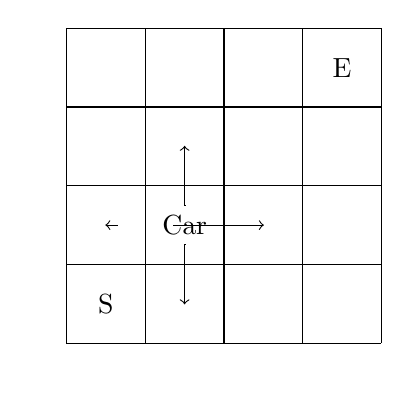
\begin{tikzpicture}[every node/.style={minimum size=1cm-\pgflinewidth, outer sep=0pt}, arrow/.style={thick}]
        \draw[step=1cm,color=black] (-2,-2) grid (2,2); 
        \node[](start) at (-1.5, -1.5) {S};
        \node[](end) at (1.5, 1.5) {E};
        \node[](car) at (-0.5, -0.5) {Car};
        
        \node[](car_up_center) at (0.0, -0.25) {};    
        \node[](car_up) at (-0.5, 1.0) {};
        
        \node[](car_down_center) at (0.0, -0.75) {};
        \node[](car_down) at (-0.5, -2.0){};
    
        \node[](car_left_center) at (-1.35, -0.5) {};
        \node[](car_left) at (-2.0, -0.5){};
    
        \node[](car_right_center) at (-0.65, -0.5) {};
        \node[](car_right) at (1.0, -0.5){};
        
        % \node[](charge site) at (-0.5, 1.5) {$t_{1}$};
        % \node[](charge site) at (1.5, -0.5) {$t_{2}$};
        \draw[->, to path={-| (\tikztotarget)}]
     	( car_up_center) edge (car_up)  (car_down_center) edge (car_down) ;
         \draw[<-, to path={-| (\tikztotarget)}]
     	(car_left) edge (car_left_center) (car_right) edge (car_right_center);
    \end{tikzpicture}
    \caption{场景1:简单网格地图}
    \label{figcase1}
\end{figure}

\subsection{场景2:带有转弯惩罚的场景}
在现实交通网络中,对最短路径计算结果具有重要影响的因素之一为转弯方向的选择,例如在图\ref{figcase1}实例中,同时存在多条从起点到终点的最短路径,但在实际交通网络中,例如中国等靠右行驶的国家中,左转往往比直行和右转具有更长的时间消耗。因此在两条最短路径行驶长度完全相同的情况下,较少左转的路径往往实际消耗的时间更少。
我们通过加入额外的转弯惩罚设计了场景2,在该场景中,在任意一条边上的移动损失函数定义为式\ref{case2movingcost},其中$A \in\mathbb{R}, C\ge0$为常数,表示转弯的额外惩罚。
\begin{equation}
\label{case2movingcost}
f(e_{v_i,v_{i+1}}) = \begin{cases}
C + A &\mbox{if car turn left or turn around}\\
C &\mbox{else}
\end{cases}
\end{equation}

\subsection{场景3:带有行驶路径限制和充电桩的场景}
随着电动汽车的普及和推广,基于电动车的路径规划也作为某一特定问题被各国学者进行研究。该场景的特殊性在于,电动车普遍行驶距离较短,在进行单次路径规划中,我们在求解最短路径的同时,需要保证其在任意行驶过程中保持电量大于零,如果电量过低,需要到就近的充电桩进行充电后再行驶。
这给原始的简单网格地图的场景带来了如下变化。\par
首先,地图中增加多个充电桩的位置,充电桩的集合被定义为 $T = \{t_{1}, t_{2}...,t_{k}\}, t_i \in V$;
同时对车辆,除去其当前位置,我们需要引入$\mathrm{power}\in[0, FULL\_POWER]$表示车辆当前剩余电量。其中 $FULL\_POWER\ge0$,表示车辆电量的最大值。修改后的地图如图\ref{figcase2}所示

\begin{figure}[H]
\centering
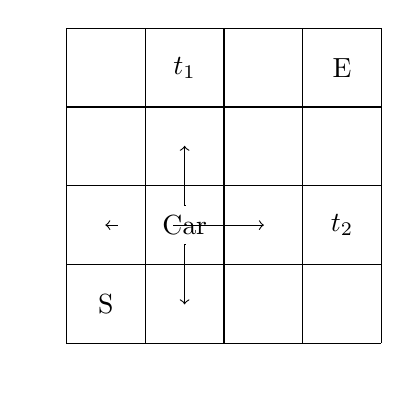
\begin{tikzpicture}[every node/.style={minimum size=1cm-\pgflinewidth, outer sep=0pt}, arrow/.style={thick}]
    \draw[step=1cm,color=black] (-2,-2) grid (2,2); 
    \node[](start) at (-1.5, -1.5) {S};
    \node[](end) at (1.5, 1.5) {E};
    \node[](car) at (-0.5, -0.5) {Car};
    
    \node[](car_up_center) at (0.0, -0.25) {};    
    \node[](car_up) at (-0.5, 1.0) {};
    
    \node[](car_down_center) at (0.0, -0.75) {};
    \node[](car_down) at (-0.5, -2.0){};

    \node[](car_left_center) at (-1.35, -0.5) {};
    \node[](car_left) at (-2.0, -0.5){};

    \node[](car_right_center) at (-0.65, -0.5) {};
    \node[](car_right) at (1.0, -0.5){};
    
    \node[](charge site) at (-0.5, 1.5) {$t_{1}$};
    \node[](charge site) at (1.5, -0.5) {$t_{2}$};
    \draw[->, to path={-| (\tikztotarget)}]
 	( car_up_center) edge (car_up)  (car_down_center) edge (car_down) ;
     \draw[<-, to path={-| (\tikztotarget)}]
 	(car_left) edge (car_left_center) (car_right) edge (car_right_center);
\end{tikzpicture}
\caption{场景3:电动车路径规划问题的网格地图}
\label{figcase2}
\end{figure}
\section{现有的基于搜索的算法}
\subsection{Dijkstra 算法}
Dijkstrea 算法由荷兰计算机科学家 Edsger Wybe Dijkstra在1956年提出的单源最短路径算法,在随后的几年内被正式发表\citing{Dijkstra}。
\subsubsection{算法描述}
首先定义我们起始的点为$v_s$,令$D_{v_j}$表示点$v_j$到初始点 $v_s$的距离。Dijkstra 算法首先赋予一些初始距离值,然后通过迭代计算和优化距离值,算法的基本流程如下。\par
第一步,首先将所有点标记为未访问过,并放入一个未访问的点的集合$Q$中,然后对初始点,设置它的距离值$D$为0,剩余点设置为无穷大。
第二步,从未访问集合$Q$中取出具有最小距离值的点,查询它的邻居节点的距离值,
如果邻居节点通过当前节点后其距离值降低,则更新邻居节点的距离值,这一步操作成为松弛操作。当前节点的所有邻居都被更新后,将当前节点标记为已访问,然后重复第二步,直到未访问集合为空。
第三步,如果目标节点被标记为已访问,则表示我们找到了一条从起点到目标节点的最短路径。
在计算过程中,我们可以对每个点维护一个前驱节点值,即当前节点的距离值被某个邻居节点的距离值更新时,同时更新该前驱值为对应邻居节点。在计算结束后,可以通过该前驱节点值递归的输出最短路径。
\subsubsection{复杂度分析}
Dijkstra 算法的时间复杂度上下界可使用大$O$符号,由用点集$V$和边集$E$组成的函数表示,时间复杂度的上下界的紧致程度或长数值大小由算法中$Q$集合的实现决定。Dijkstra复杂度为$O(|V|^2)$,其中$|V|$为图中点的数量。但一个更精确的表述为 $O(|E|\cdot T_{dk} + |V|\cdot T_{em})$,其中$T_{dk}$表示完成集合中键的降序排列时间复杂度,$T_{em}$表示从集合中取出最小键值的时间复杂度。
\subsubsection{Dijkstra的相关改进算法}
在 Dijkstra 算法被提出后,许多基于 Dijkstra 的优化算法被提出。
由于在 Dijkstra 算法中很重要的一步为从$Q$集合中取出具有最小距离值$D$的节点,因此Boas等人提出了基于优先队列实现的改进算法,使得其复杂度降到了$O(|V|loglog|V|)$。
Fredman和 Tarjan通过斐波那契堆实现的算法复杂度为$O(|E| + |V|log|V|)$\citing{Fredman1984Fibonacci}。
\subsection{Floyd 算法}
Floyd 算法为 Robert Floyd 在1962年提出\citing{Floyd1962Algorithm},同年代,Warshall 也提出了类似算法,因此该算法又被称为 Floyd-Warshall 算法。Floyd 解决了多源最短路问题,其时间复杂度为$O(|V|^3)$,它通过枚举任意两点之间可能的最短路径然后按照基于动态规划的思想进行更新。
\subsubsection{算法描述}
设$D_{i,j,k}$表示从顶点$i$ 到顶点$j$的只以$(1..k)$集合中的节点为中间节点的最短路径长度,那么我们可以通过枚举$k \in \{1..|V|\}$,按照如下公式更新$D_{i,j,k}$:\begin{equation}
    D_{i,j,k} = min(D_{i,j,k-1}, D_{i,k,k-1} + D_{k,j,k-1})
\end{equation}

\subsection{Bellman-Ford 算法}
Dijkstra和 Floyd 算法存在的问题在于无法处理带有负环的图的最短路径问题,即如果在给定的图中,如果存在一个环路,通过该环路的损失为负值,那么理论上可以无限的降低总损失值,因而无法给出正确的最短路径。所以Richard Bellman 和 Lester Ford于1958年年提出了可以处理负环的 Bellman-Ford 算法\citing{Bellman1958On}。
\subsubsection{算法描述}
与 Dijkstra 算法类似,Bellman-Ford也是基于松弛操作,然而 Dijkstra 是通过贪心的选择距离最小的点进行松弛操作,而后者是简单的通过枚举边然后对边上的两个端点进行松弛操作,这一过程共进行$|V|-1$次,由于任意一个图上的最短路径长度不会超过$|V|-1$。
因此在$|V|-1$次松弛操作后,理论上保证了在解存在情况下,算法能够找到最短路径的解。最后 Bellman-Ford 算法通过第$|V|$次松弛操作,检测是否存在负环,如果在第$|V|$次松弛操作时,仍然存在可被缩小的距离值,那么说明负环存在。
\subsection{$A^{*}$ 算法}
$A^{*}$ 算法是一类重要的启发式搜索算法\citing{Astar},它的核心思想在于,通过对搜索的状态空间中的每一个搜索位置按照某一启发式函数进行评估,选择具有最优值的搜索点进行下一步搜索。
由于路径规划问题本质上一个在图上的搜索问题,因此$A^{*}$ 算法也被应用到了该问题中。
\subsubsection{算法描述}
在$A^{*}$ 算法中,最重要的为设计启发式函数$f(v_i)$,或者成为估算函数。一般函数具有$f(v_i) = g(v_i) + h(v_i)$的形式,其中$g(v_i)$表示从初始点走到 $v_i$的代价值,$h(v_i)$表示从点$v_i$到目标点的估计距离。在实际的算法中,我们会维护关于$g(v_i)$的表,对于$h(v_i)$,我们一般使用欧几里得距离,曼哈顿距离或切比雪夫距离等计算方法作为估算函数。\par
算法的基本流程如下,首先定义集合$C_{set}$为被估算的节点集合,$O_{set}$为将要被估算的节点集合,初始时只包括起点。起点的 $g$函数值为0,$h$函数值设为某一距离函数下的计算结果。当$O_{set}$不为空时,我们取出其中$f$值最小的点$v_{min}$,枚举该点的邻居$v_{neighbor_i}$,如果该点不在$C_{set}$中,根据松弛操作判断$v_{neighbor_i}$的$g$值是否在通过$v_{min}$后更小,如果是,则更新$v_{neighbor_i}$的$g, h, f$值,同时将$v_{neighbor_i}$加入$O_{set}$,如果否,则不做任何更新和操作。最终当我们取出的点$v_{min}$为目标点时,说明我们找到了解。
\subsubsection{复杂度分析}
$A^{*}$ 算法的复杂度依赖于启发式函数的设计。在最坏情况下,$A^{*}$的复杂度相当于一个不带任何优化和限制的搜索算法的复杂度 $O(b^d)$,其中$b$为状态空间的宽度,即每个搜索状态的后继状态的平均数量,在该问题中为每个节点相临节点的数量,$d$为搜索空间的深度,在该问题中为路径的长度的最大值,即为定点的个数。而一个好的启发式函数可以大大减少搜索状态的数量,特别是$b$的值。作为搜索算法,复杂度的定义显然与搜索节点的数量成正比,因此我们定义 $N$: 
    \begin{equation}
        N + 1 = 1 + b^* + (b^*)^2 + ... + (b^*)^d
    \end{equation}
而最优的启发式函数$h_*(x)$具有$b=1$。对于任意一个非最优的启发式函数,当其启发式函数符合方程\ref{eq3astar},其时间复杂度为多项式级别。
    \begin{equation}
    \label{eq3astar}
        |h(x) - h_*(x)| = O(logh_*(x))
    \end{equation}
\subsection{改进算法}
随着交通网络的复杂度提高,基于图的搜索算法难以处理过大的地图,因此一些优化方法便被提出。\par
Thorup 和 Zwick 提出了基于预处理和查询的分步方法\citing{Thorup2001Compact}。这类方法首先离线对原始图进行预处理,降低原问题的复杂度,然后在查询阶段,利用预处理阶段得到的数据和简化后的图快速给出路径规划结果。
第二类改进算法为结构化的最短路径算法,交通网络本身具有一定的结构性质,即分层模型,通过将地图按照一定的规则分层,然后对分层后的模型做路径规划可以提升原有算法的性能。例如 Sanders 和 Schultes 提出了通过定义邻近集合和邻近搜索的方法\citing{Sanders2005Highway, Sanders2006Engineering},这类方法被称为公路结构化方法(Highway Hierarchies)方法。同样 Geisberger 等人提出了基于缩点的结构化方法\citing{Geisberger2008Contraction},通过对节点按照重要性排序,然后将非重要的节点进行缩点和替换从而减小图的规模。\par
Delling等人提出了可定制化的最短路径算法\citing{Delling2011Customizable},他们将图分为静态的拓扑结构,包括了边,节点等,和计算模式,即如何计算行驶损失的方法两部分。使得前者维持静态,后者为一个动态模块。该算法分为三个步骤,首先为独立损失计算部分,在这一步只对静态图进行预处理,第二步为定制化计算损失阶段,对不同的损失计算方法进行处理。最后为查询阶段,根据不同的损失计算方法给出结构。

\section{本章小结}
作为本文的正式内容的第一个章节,我们给出了路径规划问题的定义,以及出现的多个新的场景和需求。通过给出严格定义,将为下面章节我们使用强化学习解决问题提供较严格的数学形式支持。同时给出了传统的基于图的搜索算法,包括经典的 Dijkstra 算法和近些年各国学者提出的种种改进算法,但我们也看到了这些算法存在的部分问题。现有的算法,大多是基于不同场景的定制化算法,对于不同的最短路计算函数,需要单独设计不同的算法,这导致不同场景下的算法具有较少的通用性和可扩展性。其次随着交通场景的复杂化和规模增大,现有的改进算法大多基于较为简单的预处理来增加额外的信息和降低图的规模。因此我们将尝试使用强化学习解决这些问题,并为路径规划问题未来的设计和发展提供新的思路。
\end{document}